%%%%%%%% CS 886 final project report (ICML 2026 template) %%%%%%%%
% Build:  latexmk -pdf main.tex
% Figures and Table 1 are generated by code/make_figures.py from results/.

\documentclass{article}

\usepackage{microtype}
\usepackage{graphicx}
\usepackage{booktabs}
\usepackage{hyperref}

\newcommand{\theHalgorithm}{\arabic{algorithm}}

% [preprint] prints the author name (a course report is not blind-reviewed).
\usepackage[preprint]{icml2026}

\usepackage{amsmath}
\usepackage{amssymb}
\usepackage{mathtools}
\usepackage{xcolor}
\usepackage[capitalize,noabbrev]{cleveref}

% Placeholder marker. Search for "TODO" before submitting.
\newcommand{\TODO}[1]{\textcolor{red}{[TODO: #1]}}
\newcommand{\Nprob}{N}      % number of training problems
\newcommand{\Bud}{B}        % budget of labelled steps
\newcommand{\shown}{$\bullet$}
\newcommand{\hidden}{$\circ$}
\newcommand{\Bfifty}{B_{50}}

\icmltitlerunning{Complete vs.\ Partial Chain-of-Thought Traces under a Fixed Budget}

\begin{document}
\raggedbottom % put leftover space at the bottom of a column, not between paragraphs

\twocolumn[
  \icmltitle{Complete vs.\ Partial Chain-of-Thought Traces\\
    under a Fixed Budget}

  \begin{icmlauthorlist}
    \icmlauthor{Anurag Chakraborty}{}
  \end{icmlauthorlist}

  \icmlkeywords{chain of thought, sample complexity, transformers, sparse parity, multiplication}

  \vskip 0.3in
]

\makeatletter\global\icml@noticeprintedtrue\makeatother

%-----------------------------------------------------------------------
\begin{abstract}
Training on intermediate steps (chain of thought, CoT) lets transformers learn
tasks that are hard to learn from the final answer alone. However, labelling
every step of every training problem is expensive. We study how best to
allocate a fixed budget of labelled steps: complete traces for a few problems,
or partial traces for many. We train small transformers from scratch on sparse
parity and on multiplication of two 4-digit numbers, and spend the same budget
in three ways: complete traces, random partial traces that label a fraction
$q$ of all steps, and periodic partial traces that label every $(1/q)$-th
step. At test time, the model receives only the input and must write the
entire trace. We test the locality-based prediction that a step is learned
only from problems that also show the step before it. Random traces contain a
fraction $q$ as many such neighbouring pairs and need about $1/q$ times the
budget of complete traces, for every $q$ on parity and for $q\ge\tfrac12$ on
multiplication (at $q=\tfrac14$, optimization failures raise the cost).
Periodic traces contain no neighbouring pairs and almost never succeed, even
though the models fit the steps they are shown.
\end{abstract}

%-----------------------------------------------------------------------
\section{Introduction}
\label{sec:intro}

Labelling reasoning traces is a major cost of CoT training. Given a budget of
$\Bud$ labelled steps, one can label complete traces for a few problems or
partial traces for many. In large language models, truncated or
endpoint-only traces keep most of the benefit of full traces
\citep{hwang2026revisiting,chen2025distilling}, which these studies attribute
to redundancy in long natural-language traces. It remains open whether
partial traces also work when every step is needed.

The locality view of CoT \citep{wen2025sparse,abbe2024globality} holds that a
step is easy to learn when it depends on only a few visible tokens. For
partial traces, this suggests that a step is learnable only when the step
before it is also visible. We test this prediction in a controlled,
budget-matched setting. Our contributions are empirical:
(i) a budget-matched comparison of complete, random and periodic traces on
two tasks, scored by whether the model writes the whole trace,
(ii) $P$, the number of training problems that show a step together with the
step before it, which predicts that random traces need about $1/q$ times the
budget of complete traces, and
(iii) evidence that steps after a gap do not help, even when easy to learn,
and that periodic traces fail even when the models fit the steps they are
shown.

%-----------------------------------------------------------------------
\section{Background}
\label{sec:background}

\paragraph{Parity.}
Learning a $k$-sparse parity of $n$ bits from the final answer label needs about
$n^{k}$ computation with gradient-based training, because no smaller set of
input bits is correlated with the answer \citep{barak2022hidden}. The intermediate
CoT trace removes this difficulty: when the running parity is written out, each
step depends on only two tokens, the previous step and one input bit, and
transformers require far fewer samples to learn in this setup \citep{wen2025sparse}.

\paragraph{Multiplication.}
Without intermediate steps, small transformers trained in the standard way
fail to multiply two 4-digit numbers \citep{deng2023implicit,deng2024explicit}.
\citet{bai2025multiplication} trace this to long-range dependencies between
digits and show that training the model to predict the intermediate running sum
solves this issue. Closest to partial traces, \citet{deng2024explicit} remove CoT tokens
gradually during training, a schedule rather than the fixed partial traces
studied here.

%-----------------------------------------------------------------------
\section{Setup}
\label{sec:setup}

\paragraph{Tasks.}
\emph{Parity:} the input is $n$ random bits ($n=30$ unless stated), and the answer
is the XOR of a secret subset of $k=8$ positions, fixed per seed. Step $j$ is
the running parity after the $j$-th selected bit, so a trace has $T=8$
one-token steps and the last step equals the answer.
\emph{Multiplication:} $a\times b$ for $a$ and $b$ drawn uniformly from 4-digit
numbers, following \citet{lee2024teaching,deng2024explicit}. Step $j$
multiplies $a$ by the $j$-th digit of $b$, starting from the last digit, and
records this partial product and the running sum. For $1234\times5678$, step 2
is $(86380,\,96252)$: the product $1234\times70$ and the sum $9872+86380$. Numbers are padded to 8 digits and
written last digit first, so there are $T=4$ steps of 16 tokens each.
In both tasks a sequence is the input, a separator, the steps, an answer
marker and the answer.

\paragraph{Budget allocations.}
With $\Nprob$ training problems of $T$ steps each and a fraction $q$ of steps
shown, every case labels exactly $\Bud=q\Nprob T$ CoT steps.
\Cref{tab:arms} shows each allocation for $\Nprob=4$
problems of $T=4$ steps at $q=\tfrac12$, so $\Bud=8$.
\emph{Complete} (first row): all steps of $q\Nprob$ problems and none of the
rest (problems 1 and 2).
\emph{Random} (second row): $\Bud$ steps chosen uniformly at random from all
$\Nprob T$, so a problem can have any number of labelled steps.
\emph{Periodic} (third row): every problem shows every $(1/q)$-th step, here
every second step, starting at step 1 in half of the problems and at step 2
in the other half. Each step is then shown in a fraction $q$ of problems,
but two neighbouring steps are never shown together.
Hidden steps are replaced by blank tokens, so every step keeps its position.

\begin{table}[h]
  \caption{Budget $\Bud=8$, $\Nprob=4$ problems, $T=4$ steps,
  $q=\tfrac12$ (\shown\ shown, \hidden\ hidden).}
  \label{tab:arms}
  \centering\small
  \begin{tabular}{@{}lcccc@{}}
    \toprule
    Problem  & 1 & 2 & 3 & 4 \\
    \midrule
    Complete & \shown\shown\shown\shown & \shown\shown\shown\shown & \hidden\hidden\hidden\hidden & \hidden\hidden\hidden\hidden \\
    Random   & \shown\hidden\shown\shown & \hidden\shown\hidden\hidden & \shown\shown\hidden\hidden & \hidden\shown\shown\hidden \\
    Periodic & \shown\hidden\shown\hidden & \hidden\shown\hidden\shown & \shown\hidden\shown\hidden & \hidden\shown\hidden\shown \\
    \bottomrule
  \end{tabular}
\end{table}

\paragraph{Model and training.}
We train decoder-only pre-norm transformers with learned positional
embeddings from scratch, with next-token loss on the shown steps and the
answer. Parity uses width 64, 2 layers and 2 heads (0.1M parameters),
and multiplication uses width 128, 4 layers and 4 heads (0.8M parameters).
We use AdamW with learning rate $10^{-3}$ (linear warm-up over 1{,}000
updates, then constant), weight decay 0.1 and
$\beta=(0.9,0.98)$, batch size 256, gradient clipping at norm 1, and at most
40{,}000 updates.

\paragraph{Test accuracy.}
At test time the model is given only the input and must write every step and
the answer itself, on 1{,}000 (parity) or 500 (multiplication) fresh
problems. Its exact accuracy is the fraction of problems with every token
right, measured every 500 (parity) or 1{,}000 (multiplication) updates.

\paragraph{Budget needed.}
A \emph{run} is one trained model, for one allocation, $q$, training-set size
$\Nprob$ and seed. A run \emph{succeeds} if its exact accuracy is at least
95\% at three consecutive measurements. For each allocation and $q$ we train 3 runs
(9 for multiplication at $q=\tfrac14$) at every training-set size. The sizes
go from 62 to 32{,}000 problems for parity and from 700 to 128{,}000 for
multiplication, each a factor of $\sqrt2$ larger than the one before.
We treat every run as a pass or a fail and fit one logistic curve, over all sizes and seeds, for the
probability that a run succeeds as a function of $\log\Nprob$. The
\emph{budget needed}, $\Bfifty$, is the number of labelled steps at which
this fitted probability is one half. For example, for Complete on parity at
$q=\tfrac12$, 1 of 3 runs succeeds with 500 labelled steps and 2 of 3 with
708, and the fitted curve reaches one half at 595. 
Two allocations are compared by dividing their budgets needed,
with a 90\% bootstrap interval for this ratio (\cref{tab:b50}).

%-----------------------------------------------------------------------
\section{Prediction}
\label{sec:predictions}

Let $s_j$ be step $j$ of parity and $S_j$ the running sum in step $j$ of
multiplication. If step $j{-}1$ is shown, step $j$ depends on it and one new
input token:
\begin{align*}
s_j &= s_{j-1}\oplus x_{i_j}, & S_j &= S_{j-1}+a\,b_j\,10^{j-1}.
\end{align*}
If the $g$ steps before it are hidden, it depends on $g{+}1$ new input tokens:
\begin{align*}
s_j &= s_{j-g-1}\oplus x_{i_{j-g}}\oplus\cdots\oplus x_{i_j},\\
S_j &= S_{j-g-1}+a\textstyle\sum_{i=j-g}^{j} b_i\,10^{i-1}.
\end{align*}
In parity these bits are at unknown positions, and such a step takes about
$n^{g+1}$ computation to learn \citep{barak2022hidden,abbe2024globality}. In
multiplication the digits of $b$ are at known positions, which makes such a
step easier to learn.

Assume that at our budgets steps shown after a gap do not help. Then step $j$
is learned only from problems that show steps $j{-}1$ and $j$ together. The
number of such problems is $P=q\Nprob$ for Complete, $P\approx q^2\Nprob$ for
Random, which shows each step with probability $q$, and $P=0$ for Periodic.
At equal budget, Random thus has only a fraction $q$ as many pairs as
Complete. This gives three predictions:
\textbf{(P1)} Success depends on $P$ alone: Complete and Random coincide when
plotted against $P$, and Random needs $1/q$ times the budget.
\textbf{(P2)} Periodic fails at every budget.
\textbf{(P3)} If steps after a gap do help, Random needs less than $1/q$
times the budget and Periodic starts to succeed. This would appear first where
a step after a gap is easiest to learn: in parity with small $n$, and in
multiplication.

%-----------------------------------------------------------------------
\section{Results}
\label{sec:results}

\begin{figure*}[t]
  \centering
  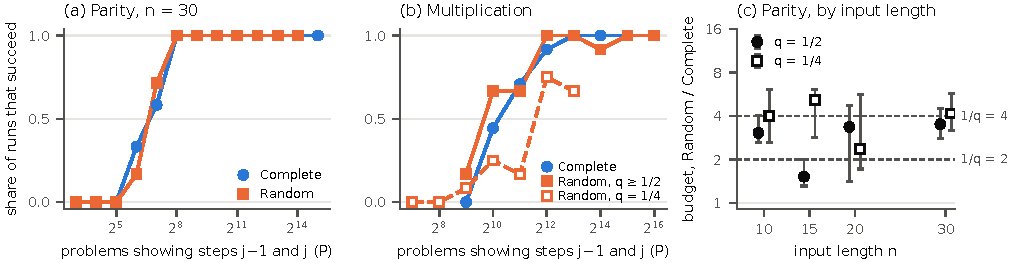
\includegraphics[width=\textwidth]{figures/results.pdf}
  \caption{\textbf{(a, b)} Share of runs that succeed against $P$, the number
  of training problems that show a step together with the step before it.
  Each point pools all $q$ and all runs whose $P$ lies within the same factor
  of 2. Complete and Random fall on one curve, except Random at $q=\tfrac14$
  in multiplication. Periodic has $P=0$ and is not shown (\cref{tab:b50}).
  \textbf{(c)} Parity: budget needed by Random divided by that of Complete,
  against input length $n$, with 90\% intervals. Dashed lines mark the
  prediction $1/q$.}
  \label{fig:results}
\end{figure*}

\begin{table}[t]
  \caption{Budget needed $\Bfifty$ (labelled steps), the ratio Random/Complete
  (measured with 90\% interval, and predicted $1/q$), and successful Periodic
  runs (Periodic is not run at $q=\tfrac34$).}
  \label{tab:b50}
  \centering\small
  \setlength{\tabcolsep}{3.5pt}
  \begin{tabular}{@{}lrrlrr@{}}
\toprule
 & \multicolumn{2}{c}{Budget needed} & \multicolumn{2}{c}{Random / Complete} & Periodic \\
\cmidrule(lr){2-3}\cmidrule(lr){4-5}
$q$ & Complete & Random & measured & predicted & succeeded \\
\midrule
\multicolumn{6}{@{}l}{\emph{Parity, $n=30$}} \\
3/4 & 793 & 1,405 & 1.8 [1.6, 2.2] & 1.3 & -- \\
1/2 & 595 & 2,088 & 3.5 [2.8, 4.5] & 2.0 & 0 of 45 \\
1/4 & 903 & 3,759 & 4.2 [3.2, 5.7] & 4.0 & 0 of 45 \\
1/8 & 1,053 & 5,971 & 5.7 [4.0, 8.0] & 8.0 & 1 of 45 \\
\midrule
\multicolumn{6}{@{}l}{\emph{Multiplication, 4 digits by 4 digits}} \\
3/4 & 3,901 & 4,771 & 1.2 [0.8, 2.0] & 1.3 & -- \\
1/2 & 4,686 & 8,940 & 1.9 [1.0, 3.8] & 2.0 & 0 of 39 \\
1/4 & 7,733 & 52,695 & 6.8 [4.6, 11.5] & 4.0 & 0 of 39 \\
\bottomrule
\end{tabular}

\end{table}

\paragraph{Parity (P1, P2).}
For all four values of $q$, the success curves of Complete and Random
coincide when plotted against $P$ (\cref{fig:results}a), as (P1) predicts.
At their budget needed, both allocations have about a hundred pairs per step:
$P=75$--130 for Complete and $P=90$--130 for Random. Measured in labelled
steps, Random needs 1.8, 3.5, 4.2 and 5.7 times the budget of Complete at
$q=\tfrac34,\tfrac12,\tfrac14,\tfrac18$, against the predicted 1.3, 2, 4 and
8 (\cref{tab:b50}). The measured ratios are within a factor of two of the
prediction, higher at large $q$ and lower at $q=\tfrac18$. Periodic, which
shows each step as often as Random but has $P=0$, succeeded in 1 of 135
runs, as (P2) predicts.

\paragraph{Parity at shorter inputs (P3).}
At $n=10$, a step after one hidden step is a parity of 2 of 10 bits, against
2 of 30 at $n=30$. However, the ratio Random/Complete is 3.1 at $q=\tfrac12$ and 4.0
at $q=\tfrac14$ for $n=10$, and 3.5 and 4.2 for $n=30$
(\cref{fig:results}c). Over all $n$, its geometric mean is 2.7 at
$q=\tfrac12$ and 3.8 at $q=\tfrac14$. Periodic failed in all 90 runs at
$n\le20$. Its runs with $\Nprob\ge8{,}000$ reach a median final training loss
below 0.001 and still fail at test time. This shows that steps after a gap
do not help at our budgets, even when they are easier to learn and the
model fits them.

\paragraph{Multiplication (P1--P3).}
For $q\ge\tfrac12$, the success curves of Complete and Random coincide when
plotted against $P$ (\cref{fig:results}b). Random needs 1.2 and 1.9 times the
budget of Complete at $q=\tfrac34$ and $\tfrac12$, against the predicted 1.3
and 2. Both allocations need about 900--1{,}900 pairs per step, ten times more than
in parity. At $q=\tfrac14$, Random needs 6.8 times the budget of Complete,
against the predicted 4, and many of its runs stall below 15\% exact
accuracy (8 of 9 at $\Nprob=8{,}000$, 1 of 9 at $\Nprob=64{,}000$). Periodic
failed in all 78 runs, with at most 1\% correct answers. This shows that for
$q\ge\tfrac12$, $P$ predicts the cost of Random in multiplication as
well, and that steps after a gap do not help, even though they
are easier to learn than in parity. At $q=\tfrac14$, stalled runs make Random cost
more than $P$ predicts.

%-----------------------------------------------------------------------
\section{Discussion and limitations}
\label{sec:discussion}

The budget ordering is consistent with the locality view and with $P$:
Complete needs the least budget, Random about $1/q$ times as much (within a
factor of two for parity and for multiplication with $q\ge\tfrac12$), and
Periodic, with $P=0$, almost always fails. Periodic also shows that fitting
the supervised steps is not enough to write the full trace. Its training
never shows a step together with the step before it, while at test time the
step before it is always visible. We cannot tell whether the models never
learn to compute a step from its predecessor, or learn it in the periodic
context but fail to apply it at test time. Our results suggest that when only
part of each trace can be labelled, the labelled steps should include
consecutive ones.

\paragraph{Limitations.}
Models are small and trained from scratch on two synthetic tasks with no redundant steps, unlike the long natural-language traces for which partial supervision has 
been reported to work \citep{hwang2026revisiting}. Hidden steps are blanked rather than deleted, and training is capped at 40{,}000 updates. Estimates of the required 
budgets are based on 3 seeds per size (9 for multiplication at $q=\tfrac14$). For $n\le20$, we also use a coarser set of sizes, resulting in wider intervals for the 
ratios. The evaluation requires the full trace by design. If evaluated only by their answers, partial-trace models may rank differently.

%-----------------------------------------------------------------------
\section*{Software and Data}
Code, results and the scripts for \cref{fig:results} and \cref{tab:b50}:\\
\url{https://github.com/anuchak/CS-886-Course-Project} (commit \texttt{e81bf5f}).

\bibliography{refs}
\bibliographystyle{icml2026}

\end{document}
